\newpage
\section{Introduction}
\label{intro}

Main memory sizes have grown significantly to the degree that 
they can hold big chunks of data main-memory resident, often all the data of modern database instances.
This has lead to an increased attention towards main-memory tailored techniques.
Even though data can be accessed fast in main-memory, e.g., with scans over dense arrays, still 
proper indexing provides significant benefits for range or point queries.

Past research has shown that main-memory tailored indexing techniques can significantly outperform
standard techniques such as binary search over a dense sorted array \cite{cbbtrees,art}.


\begin{figure}[t]
\center
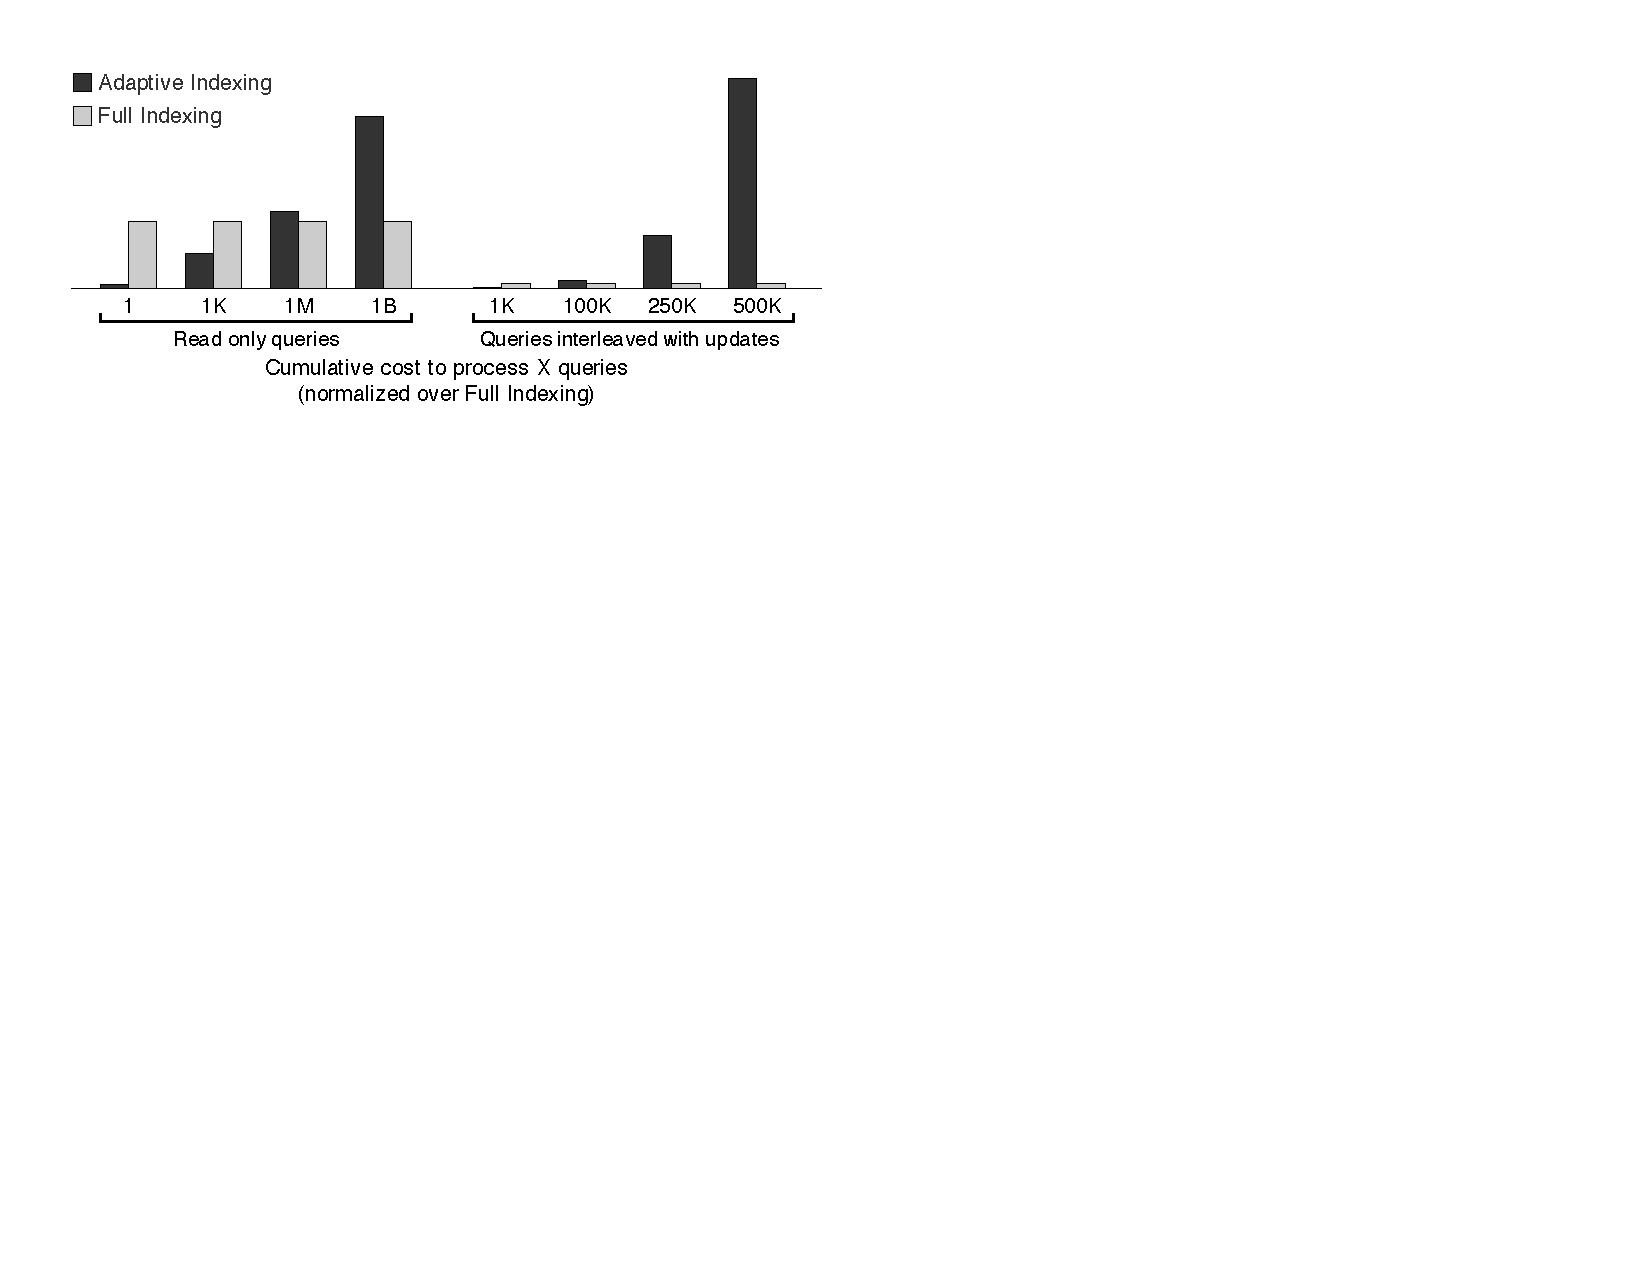
\includegraphics[width=0.85\columnwidth]{graphs/motivation.pdf}%
%\vspace{-1.5em}
\caption{The need for transitive indexing: A different design is best for different stages of a workload.}
%\vspace{-2.5em}
\label{F:Motivation}
\end{figure}

\textbf{The Problem: Read-write Intensive Workloads.}
In this paper, we address the need of modern applications to handle workloads which require both efficient read and efficient update
support in the same system. 
There is an increasing attention to this problem at various levels, e.g., 
in terms of database architectures with efforts such as SAP HANA \cite{Hana} and Hyper \cite{hyper} or also at the indexing level
with efforts such as ART main-memory indexing \cite{art}.
A problem with traditional  static indexing approaches is that one has to know exactly which data should be indexed
and then also have the time and resources to go through a very expensive indexing phase.
As applications become more and more real-time and with ad-hoc querying demands, such static approaches
become a bottleneck to having a quick access to new data.
A number of adaptive indexing approaches have been proposed lately to address exactly this problem of static indexing \cite{IKM:CIDR07,hail}.
With adaptive indexing, indexes are built and refined incrementally during query processing
by treating each query as an advice of how data should be stored.
However, we show that although existing adaptive indexing techniques 
do provide significant improvement for ad-hoc workloads, minimizing or even eliminating initialization costs, 
they are not resilient in the same way that non-adaptive indexing is for read-write intensive workloads. 

\textbf{Motivating Example.}
Figure \ref{F:Motivation} demonstrates this problem: it depicts the relative time needed ($y$-axis) 
to answer the first X queries ($x$-axis) in a long sequence of random range 
queries and updates over a single column of $10^8$ tuples (10 updates arrive every 10 read queries). 
Each graph is normalized (independently) over its static indexing costs.
In this case, for static indexing we use the state-of-the-art in memory index ART \cite{art}
while for adaptive indexing we use the state-of-the-art stochastic cracking index \cite{StochasticCracking}.
Figure \ref{F:Motivation} shows that while early in the query sequence adaptive indexing 
significantly outperforms static indexing,
as the sequence evolves,
adaptive indexing loses its advantage over static indexing, i.e.,  it is not resilient.
The first query for adaptive indexing is more than 10 times faster than static indexing;
Full indexing needs to fully index the column, while adaptive indexing performs only small index refinement actions with every query.
However, as more queries and updates arrive, adaptive indexing eventually becomes more than 10 times slower than static indexing.

Ideally, we would like to maintain the performance of adaptive indexing early in the query sequence 
and the performance of static indexing later on.


\textbf{Contributions: Transitive Indexing.}
Our contributions are as follows.
\begin{itemize}

\item We propose a new main-memory indexing research area, termed 
\emph{transitive indexing}.
The idea is that a data structure representing an index does not have a static shape.
Instead, its shape morphs over time as the workload evolves.

\item
We present Trimmer, a transitive indexing approach which  
initially requires no preparation or initialization steps.
Data is simply appended in the form of vectors with no order forced
both inside each vector and across vectors.
As the workload evolves, Trimmer starts forcing order and structure.
Each vector is independently indexed and refined, while data starts flowing from vector to vector.
Gradually, the vectors start morphing into a Trie structure optimized for main-memory.
Only the hot part of the data morphs and everything happens during query processing
without any need for any administration or control.

\item
We show that Trimmer  maintains all the good properties of 
both existing adaptive indexing approaches and those of non-adaptive approaches, 
i.e., it is lightweight, it continuously adapts by incrementally refining indexes
and it requires zero workload knowledge and preparation costs.
At the same time it is resilient, i.e., it maintains its performance advantages
unfettered even under long strings of queries and continuous data updates;
it is geared towards continuous on-the-fly data exploration under massive updates. 

\end{itemize}

We experimentally demonstrate the advantages of Trimmer
over existing static indexing and adaptive indexing techniques. 
We use both synthetic benchmarks as well as real world data and queries.
For example, in experiments with a 4 Terabyte instance of 
data and queries from the Sloan Digital Sky Survey/SkyServer
from the astronomy domain,
we show that Trimmer can handle a combined workload of $15*10^4$ queries and $5*10^8$ updates in roughly 1 minute, while 
state-of-the-art adaptive indexing needed more than 16 hours and state-of-the-art non adaptive indexing needs ??. 

%\textbf{Paper Organization.}
%The rest of the paper is organized as follows.
%Section \ref{sec:related} discusses background and related work.
%Then, Section \ref{sec:problem} presents in detail the resilience problem of 
%existing adaptive indexing techniques and their inability to cope with the requirements
%of continuous exploration.
%Section \ref{sec:cracke} presents a series of possible patches in existing adaptive indexing
%that deal with the problem only to a certain degree
%and then it introduces CTree for full resilient and adaptive exploration.
%In Section \ref{sec:experiments}, we present a detailed experimental analysis, demonstrating the effectiveness 
%and the advantages of CTree both on synthetic and on real workloads.
%Finally, Section \ref{sec:conclusion} discusses future work and concludes the paper.

%As we enter the era of data deluge one of the main emerging patterns is the need for
%data exploration techniques \cite{SurajitSigmod2012Keynote}.
%Data arrives continuously while businesses and sciences need to continuously pose
%queries in an adaptive and interactive mode \cite{NoDBcidr,Blinkmit,ResearcherGuide,Sciborg}.
%A characteristic property in such environments is that there is little idle time and workload knowledge. 
%
%\textbf{Physical Design.}
%Good performance in database systems largely relies on proper \emph{tuning} and \emph{physical design}.
%Typically, all tuning choices happen up-front, assuming sufficient workload knowledge
%and idle time. Workload knowledge is necessary in order to determine the appropriate
%tuning actions, while idle time is required in order to perform those actions.
%Modern database systems rely on auto-tuning tools to carry out these steps, e.g.,
%\cite{CN:VLDB:97,FST88,H76,SHU:VLDB:2004,DB2DesignAdvisor}.
%

%\textbf{Dynamic Environments.}
%However, in dynamic environments, workload knowledge and idle time are scarce resources.
%For example, in scientific databases new data arrive on a daily or even hourly basis,
%while query patterns follow an exploratory path as the scientists try to interpret the data
%and understand the patterns observed; there is no time and knowledge
%to analyze and prepare a different physical design hour-by-hour or even day-by-day.
%
%Traditional indexing via tuning presents three fundamental weaknesses in such cases:
%(a) the workload may have changed by the time we finish tuning;
%(b) there may be no time to finish tuning properly;
%and (c) there is no indexing support during tuning.
%
%\textbf{Adaptive Indexing.}
%Recently, a new approach to the physical design problem was proposed,
%namely \emph{database cracking} \cite{IKM:CIDR07}. %\cite{CrackingThesis}.
%Cracking introduces the notion of continuous, incremental, partial and on-demand adaptive indexing.
%Thereby, indexes are incrementally built and refined during query processing.
%Data is physically reorganized in a continuous manner, aiming to
%match the workload, by treating each query as an advice of how data should be stored.
%
%
%\textbf{The Problem. Non-Resilient Exploration.}
%At a first glance it would seem that existing adaptive indexing approaches can cover the need
%towards adaptive exploration in the era of data deluge. 
%However, in this paper we show that 
%existing adaptive indexing techniques such as database cracking, adaptive merging and their variations
%do not cope with these new challenges. The fundamental weaknesses we identify are the inability to 
%support long strings of exploratory queries interleaved with  updates.
%Figure \ref{F:Motivation} demonstrates this problem: it depicts the relative time needed ($y$-axis) 
%to answer the first X queries ($x$-axis) in a long sequence of random select 
%queries and updates over a single column of $10^8$ tuples. 
%Each graph is normalized (independently) over its full indexing costs.
%Figure \ref{F:Motivation} shows that as the sequence evolves in the read only case,
%adaptive indexing (cracking) loses its advantage over a traditional full indexing approach, i.e.,  it is not resilient.
%The first query for cracking is more than 10 times faster than full indexing;
%Full indexing needs to fully index the column, while cracking performs only small index refinement actions with every query.
%However, as more queries arrive, cracking eventually becomes 2 times slower than full indexing.
%The performance degradation is significantly worse when continuous updates interleave with read queries
%(10 updates arrive every 10 read queries).
%In order to cope with the data deluge, 
%we would like to keep both the lightweight and the adaptive behavior of cracking for the early queries,
%while still maintaining this behavior in the long run even during continuous updates. 
%
%
%\textbf{The Solution. Comb: Resilient Adaptive Indexing.}
%In this paper, we propose a new adaptive indexing approach, termed 
%\emph{ Comb (Cracking Over Malleable Buckets)}.
%Comb maintains all the good properties of existing 
%approaches, i.e., it is lightweight, it continuously adapts by incrementally refining indexes
%and it requires zero workload knowledge and preparation costs.
%At the same time it is resilient, i.e, it maintains its performance advantages
%unfettered even under long strings of queries and continuous data updates;
%it is geared towards on-the-fly data exploration. 
%
%Comb is designed for main memory column-stores; it breaks a single column into multiple disjoint pieces
%and each piece is indexed, accessed and updated independently, while data flows from piece to piece in an adaptive way
%when the index needs to be balanced. 
%We present Comb in detail and we experimentally demonstrate its advantages
%over existing indexing and adaptive indexing techniques. 
%We use both synthetic benchmarks as well as real world data and queries.
%For example, in experiments with a 4 Terabyte instance of 
%data and queries from the Sloan Digital Sky Survey/SkyServer
%from the astronomy domain,
%we show that Comb can handle a combined workload of $15*10^4$ queries and $5*10^8$ insertions in roughly 1 minute, while 
%state-of-the-art adaptive indexing needed more than 16 hours. 
%
%\textbf{Paper Organization.}
%The rest of the paper is organized as follows.
%Section \ref{sec:related} discusses background and related work.
%Then, Section \ref{sec:problem} presents in detail the resilience problem of 
%existing adaptive indexing techniques and their inability to cope with the requirements
%of continuous exploration.
%Section \ref{sec:cracke} presents a series of possible patches in existing adaptive indexing
%that deal with the problem only to a certain degree
%and then it introduces Comb for full resilient and adaptive exploration.
%In Section \ref{sec:experiments}, we present a detailed experimental analysis, demonstrating the effectiveness 
%and the advantages of Comb both on synthetic and on real workloads.
%Finally, Section \ref{sec:conclusion} discusses future work and concludes the paper.
%





